%!TEX root = ../Thesis.tex
\chapter{Introduction}\label{cha:introduction}
%
Here's a citation: \cite{Wacker2016}. Two pictures are shown, Figures \ref{fig:morten} and \ref{fig:eps}. There's also a table: Table \ref{tab:a-table}.

\section{A Section}\label{sec:a-section}

\subsection{A Subsection}\label{ssec:a-subsection}

\subsubsection{A Subsubsection}\label{sssec:a-subsubsection}

\lipsum[2]

\begin{figure}[htbp]
  \centering
  
\includegraphics[width=.3\textwidth]{img/morten}
  \caption{Some dude}
  \label{fig:morten}
\end{figure}

\begin{figure}[htbp]
  \centering
  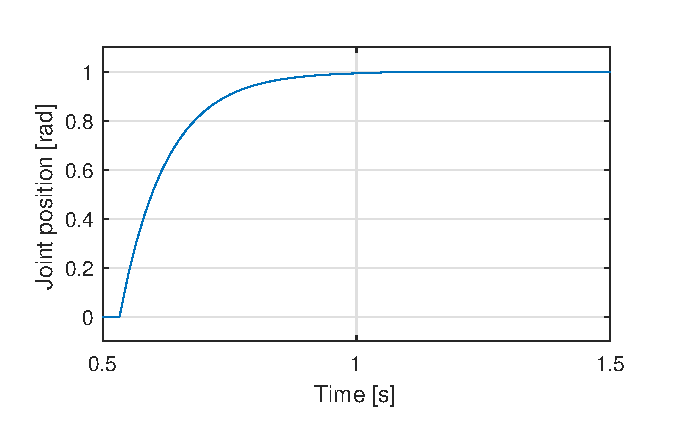
\includegraphics[width=.7\textwidth]{img/time-constant}
  \caption{An eps image}
  \label{fig:eps}
\end{figure}

\begin{table}[htbp]
  \centering
  \caption{A table}
  \begin{tabular}{cc}
    \toprule
    Something & Something else \\
    \midrule
    A & a \\
    B & b \\
    \bottomrule
  \end{tabular}
  \label{tab:a-table}
\end{table}
